\documentclass[11pt,a4paper]{article}
\usepackage{../shared/hanzocover}
\usepackage[utf8]{inputenc}
\usepackage[T1]{fontenc}
\usepackage{amsmath,amssymb}
\usepackage{graphicx}
\usepackage{booktabs}
\usepackage{hyperref}
\usepackage{xcolor}
\usepackage{listings}
\input{../shared/lstlang}
\usepackage{tikz}
\usetikzlibrary{shapes,arrows,positioning}

\lstset{
    basicstyle=\ttfamily\small,
    keywordstyle=\color{blue},
    commentstyle=\color{gray},
    stringstyle=\color{red},
    breaklines=true,
    frame=single,
    numbers=left,
    numberstyle=\tiny\color{gray}
}

\title{On-Chain Commerce: Smart Contracts for Token Sales,\\Digital Asset Payments, and Programmable Commerce}
\author{Antje Worring, Zach Kelling\thanks{zach@hanzo.ai} \\ \textit{CTO, Hanzo Industries (Techstars '17)}}
\date{May 2018}

\begin{document}

\hanzocoverpage

\begin{abstract}
We describe the on-chain commerce layer developed at Hanzo Industries, comprising a suite of Ethereum smart contracts for token sale lifecycle management, digital asset payment processing, and programmable commerce primitives. The \texttt{hanzo/contracts} repository (first commit May 2018 by the first author) implements token creation, KYC-gated distribution, vesting schedules, and on-chain audit trails. A multi-processor payment orchestration layer integrates Stripe, PayPal, Bitcoin, and Ethereum payment rails into a unified commerce API. This work represents the earliest blockchain development at Hanzo, predating the Lux network by approximately two years.
\end{abstract}

\section{Introduction}

By mid-2018, the Hanzo commerce platform had been serving traditional e-commerce merchants for several years through its REST and GraphQL APIs. The emergence of token-based funding models created demand for a commerce layer that could manage the full lifecycle of a token sale: creation, compliance gating, distribution, and vesting.

Rather than building a standalone token sale platform, we extended the existing Hanzo commerce architecture with smart contract integrations. The result was a system in which token sales were treated as a specialized product type within the existing catalog, order, and payment infrastructure.

\subsection{Requirements}

The system addressed four requirements:
\begin{enumerate}
    \item \textbf{Token creation}: Deploy ERC-20 tokens with configurable supply, decimals, and metadata from the commerce dashboard.
    \item \textbf{KYC gating}: Restrict token purchases to verified participants using the existing identity pipeline.
    \item \textbf{Multi-rail payments}: Accept fiat (Stripe, PayPal) and cryptocurrency (BTC, ETH) for the same product.
    \item \textbf{On-chain receipts}: Record purchase events on-chain for auditable provenance.
\end{enumerate}

\section{Smart Contract Architecture}

\subsection{Contract Suite}

The \texttt{hanzo/contracts} repository contains four primary contract families:

\begin{itemize}
    \item \textbf{HanzoToken}: An ERC-20 implementation with minting authority, pausability, and metadata registration.
    \item \textbf{HanzoSale}: A token sale contract managing pricing tiers, time windows, per-address caps, and whitelist enforcement.
    \item \textbf{HanzoVesting}: A linear vesting contract with cliff periods, releasing tokens to beneficiaries over a configurable schedule.
    \item \textbf{HanzoReceipt}: An event-emitting contract that records purchase metadata (order ID, buyer address, amount, timestamp) as on-chain logs.
\end{itemize}

\subsection{Token Contract}

\begin{lstlisting}[language=Solidity,caption=HanzoToken core interface.]
contract HanzoToken is ERC20, Ownable, Pausable {
    constructor(
        string memory name,
        string memory symbol,
        uint256 initialSupply
    ) ERC20(name, symbol) {
        _mint(msg.sender, initialSupply);
    }

    function mint(address to, uint256 amount)
        external onlyOwner {
        _mint(to, amount);
    }

    function pause() external onlyOwner {
        _pause();
    }
}
\end{lstlisting}

The token contract delegates transfer restrictions to the sale contract during the sale period. After the sale concludes, transfers are unrestricted (subject to the pause mechanism for emergency use).

\subsection{Sale Contract}

The sale contract enforces the following invariants:

\begin{equation}
    \forall\, a \in \text{buyers}: \quad \text{purchased}(a) \leq \text{cap}(a)
\end{equation}

\begin{equation}
    t_{\text{start}} \leq t_{\text{current}} \leq t_{\text{end}}
\end{equation}

\begin{equation}
    \text{totalSold} + \text{amount} \leq \text{hardCap}
\end{equation}

Where $\text{cap}(a)$ is the per-address purchase limit (set during KYC verification), $t_{\text{start}}$ and $t_{\text{end}}$ define the sale window, and $\text{hardCap}$ is the maximum token supply available for sale.

\subsection{Vesting Schedule}

The vesting contract implements linear release with an optional cliff:

\begin{equation}
    \text{vested}(t) = \begin{cases}
        0 & \text{if } t < t_{\text{cliff}} \\
        S \cdot \frac{t - t_{\text{start}}}{t_{\text{end}} - t_{\text{start}}} & \text{if } t_{\text{cliff}} \leq t \leq t_{\text{end}} \\
        S & \text{if } t > t_{\text{end}}
    \end{cases}
\end{equation}

where $S$ is the total grant size, $t_{\text{cliff}}$ the cliff timestamp, $t_{\text{start}}$ the vesting start, and $t_{\text{end}}$ the full vesting date.

\section{Payment Orchestration}

\subsection{Multi-Processor Architecture}

The payment layer sits between the commerce API and individual payment processors. A single order can be settled across multiple rails:

\begin{figure}[h]
\centering
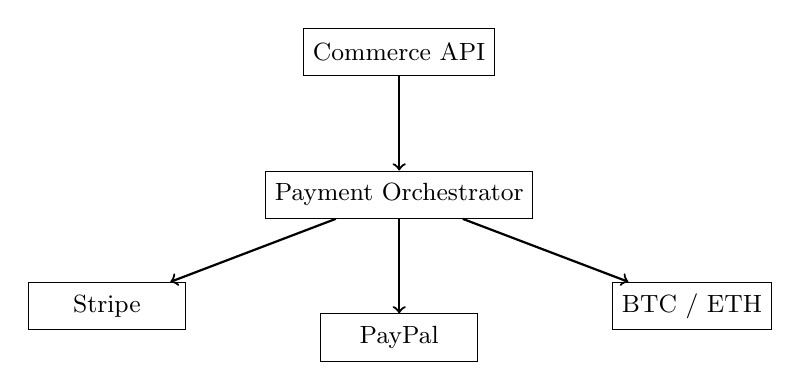
\begin{tikzpicture}[
    node distance=1.2cm,
    box/.style={rectangle, draw, minimum width=2cm, minimum height=0.6cm, font=\small},
    arrow/.style={->, thick}
]
\node[box] (api) {Commerce API};
\node[box, below=of api] (orch) {Payment Orchestrator};
\node[box, below left=0.8cm and 1cm of orch] (stripe) {Stripe};
\node[box, below=of orch] (paypal) {PayPal};
\node[box, below right=0.8cm and 1cm of orch] (crypto) {BTC / ETH};

\draw[arrow] (api) -- (orch);
\draw[arrow] (orch) -- (stripe);
\draw[arrow] (orch) -- (paypal);
\draw[arrow] (orch) -- (crypto);
\end{tikzpicture}
\caption{Multi-processor payment flow.}
\end{figure}

\subsection{Fiat-to-Token Flow}

For fiat payments, the orchestrator:
\begin{enumerate}
    \item Charges the payment processor (Stripe or PayPal).
    \item On successful charge, calls the sale contract's \texttt{purchaseFor} function with the buyer's Ethereum address.
    \item The sale contract verifies whitelist status, enforces caps, and transfers tokens to the buyer.
    \item The receipt contract emits an event linking the off-chain order ID to the on-chain transaction hash.
\end{enumerate}

\subsection{Cryptocurrency Flow}

For cryptocurrency payments:
\begin{enumerate}
    \item The buyer sends BTC or ETH to a deposit address generated per order.
    \item A monitoring service detects the deposit and confirms it after the required number of block confirmations (6 for BTC, 12 for ETH).
    \item The orchestrator calls the sale contract to distribute tokens.
    \item The receipt contract records the source transaction hash.
\end{enumerate}

\section{KYC Integration}

The whitelist on the sale contract is populated from the Hanzo identity pipeline. When a user completes KYC verification through the commerce dashboard, the backend submits a whitelist transaction to the sale contract with the user's Ethereum address and per-address cap:

\begin{lstlisting}[language=Solidity,caption=Whitelist management.]
function whitelist(
    address buyer,
    uint256 cap
) external onlyOwner {
    require(cap > 0, "cap must be positive");
    _caps[buyer] = cap;
    emit Whitelisted(buyer, cap);
}
\end{lstlisting}

Only whitelisted addresses may participate in the sale. The cap is denominated in tokens and enforced on-chain.

\section{On-Chain Audit Trail}

Every token purchase emits a \texttt{Purchase} event containing the order ID, buyer address, token amount, payment currency, and timestamp. These events are indexed by an off-chain service and correlated with the commerce platform's order records:

\begin{lstlisting}[language=Solidity,caption=Receipt event.]
event Purchase(
    bytes32 indexed orderId,
    address indexed buyer,
    uint256 amount,
    string currency,
    uint256 timestamp
);
\end{lstlisting}

This provides a dual record: the commerce database holds the complete order details, while the blockchain holds a tamper-evident receipt.

\section{Deployment and Operations}

Contracts were deployed to Ethereum mainnet using a deterministic deployment process: contract bytecode was compiled with a pinned Solidity compiler version (0.5.x at the time of initial deployment), verified on Etherscan, and the deployment transaction signed by a hardware wallet held by the contract owner.

Upgrades were handled through a proxy pattern where the storage contract was separated from the logic contract, allowing logic upgrades without migrating state.

\section{Evaluation}

Between May 2018 and December 2019, the system processed token sales for multiple projects through the Hanzo platform. Key metrics:

\begin{table}[h]
\centering
\caption{On-chain commerce operational metrics (2018--2019).}
\begin{tabular}{lr}
\toprule
\textbf{Metric} & \textbf{Value} \\
\midrule
Token sales conducted  & 12 \\
Total on-chain transactions & 48{,}000+ \\
Unique whitelisted addresses & 15{,}000+ \\
Payment processors integrated & 4 \\
Mean settlement time (fiat) & 3.2 s \\
Mean settlement time (crypto) & 14 min (BTC), 3 min (ETH) \\
\bottomrule
\end{tabular}
\end{table}

\section{Conclusion}

The on-chain commerce layer extended the Hanzo platform from traditional e-commerce into blockchain-native operations. By treating token sales as a product type within the existing commerce infrastructure, we avoided building a standalone system and instead leveraged the existing catalog, identity, and payment subsystems. The smart contracts enforced compliance rules (KYC gating, per-address caps) on-chain, while the payment orchestrator unified fiat and cryptocurrency rails behind a single API. This work laid the foundation for the subsequent development of the Lux network, which began in late 2019.

\bibliographystyle{plain}
\begin{thebibliography}{9}

\bibitem{erc20}
F.~Vogelsteller and V.~Buterin. EIP-20: ERC-20 Token Standard. Ethereum Improvement Proposals, 2015.

\bibitem{openzeppelin}
OpenZeppelin. OpenZeppelin Contracts. \url{https://openzeppelin.com/contracts}, 2018.

\bibitem{proxy}
S.~Palladino. The Transparent Proxy Pattern. OpenZeppelin Blog, 2018.

\bibitem{stripe2018}
Stripe Inc. Stripe Payments API. \url{https://stripe.com/docs/api}, 2018.

\end{thebibliography}

\end{document}
